% DOC SETTINGS ===================================
\documentclass{article}
\usepackage[utf8]{inputenc}
\usepackage{steinmetz}
\usepackage{mathtools}  
\usepackage{multicol}
\usepackage{circuitikz}
\usepackage{listings}
\usepackage{geometry}
\usepackage{indentfirst}
\usepackage{fancyhdr}
\pagestyle{fancy}
\usetikzlibrary{positioning, fit, calc}
\lhead{ECE2564 Project 2 Report}
\rhead{Kavin Thirukonda 2021}
\fancyheadoffset{0mm}
\title{Project 2 Report}
\author{Kavin Thirukonda\\
  Virginia Tech:  ECE2564\\
  Github ID: kavnthir
}
\date{April 2021}
 \geometry{
 a4paper,
 total={170mm,257mm},
 left=20mm,
 top=25mm,
 }
\mathtoolsset{showonlyrefs} 
% DOC SETTINGS ===================================
\begin{document}
\maketitle
\newpage
\section{Report Summary}
\indent
This report is meant to introduce the project, introduce the micro-controller that the project is being implemented on, and in addition talk about how the code to achieve the goals of the project is structured and organized.
\section{Project Description}
\indent
In this project, we had to develop a bee pollination game on the MSP432P401R Launchpad. This required knowledge of finite state machines, the UART terminal, C programming, joystick ADC, and the Display residing on the Booster pack board. There are five main stages of the game, the title screen, the menu screen, the play game screen, and the results screen. In addition to this there is a high score screen and a rules screen available on the menu screen. On the title screen the player is introduced to the title of the game the author, and given a short animation of a bee to introduce the concept of the game. On the menu screen the user must scroll through three options, play game, rules, and high scores. When they pick the play game screen the game starts and the player is given control of a bee, from there they must collect pollen and bring it to flowers, if an unpollinated flower touches the ground then the player loses a life. After the player loses all their lifes the results screen is shown and after a little bit they are brought to the menu screen.

\begin{center}
    \boxed{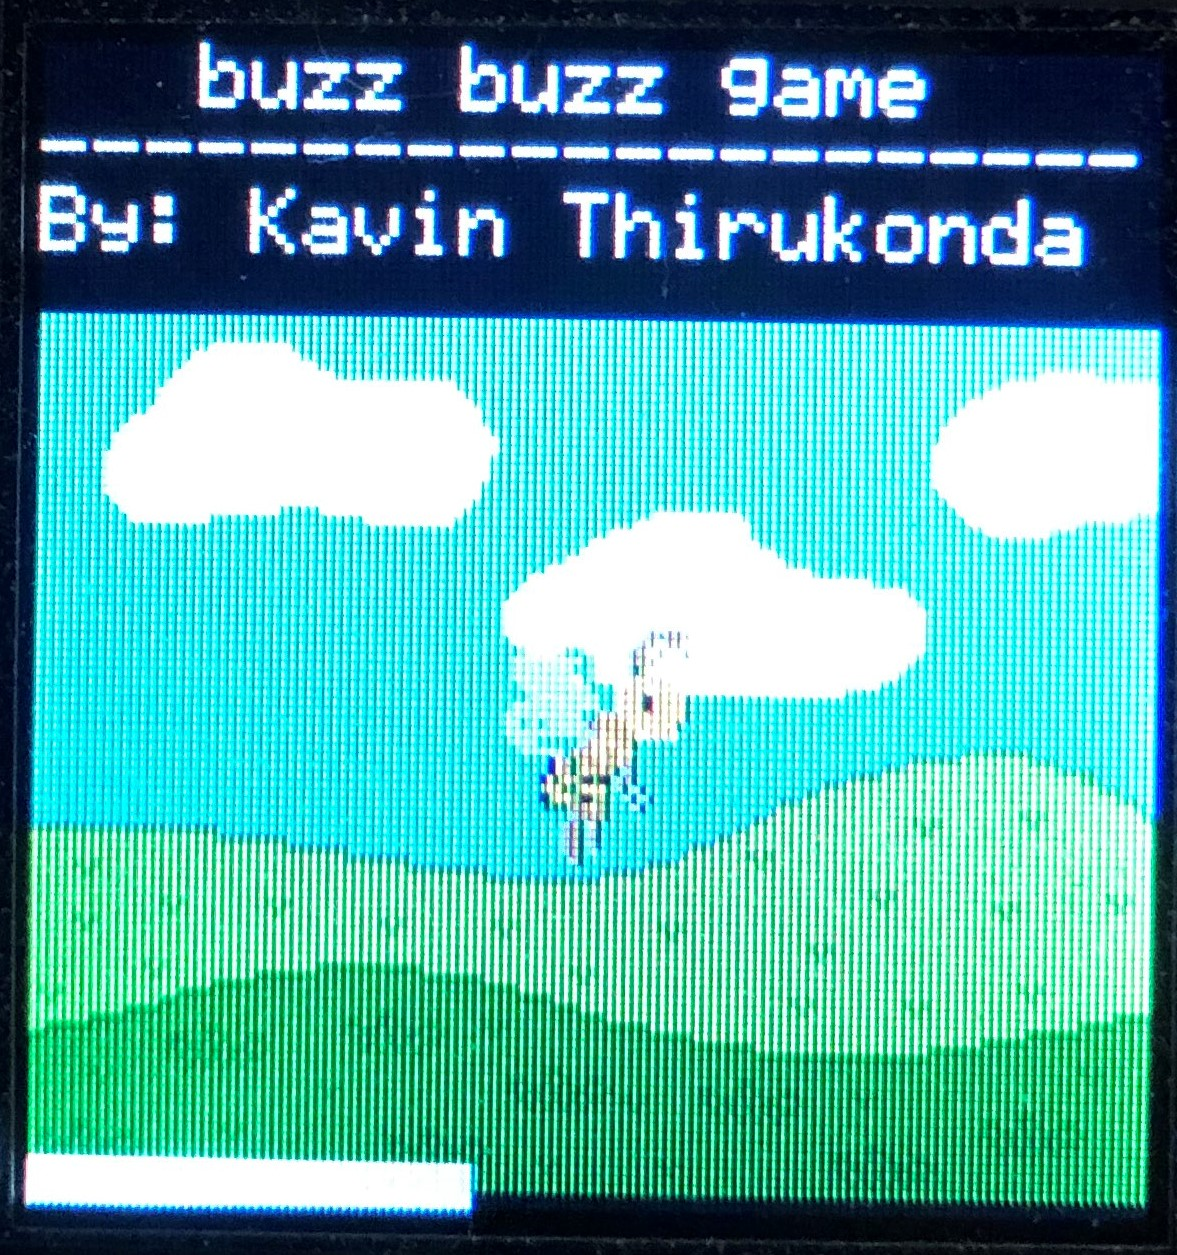
\includegraphics[width=.225\textwidth]{splash.jpg}}
    \boxed{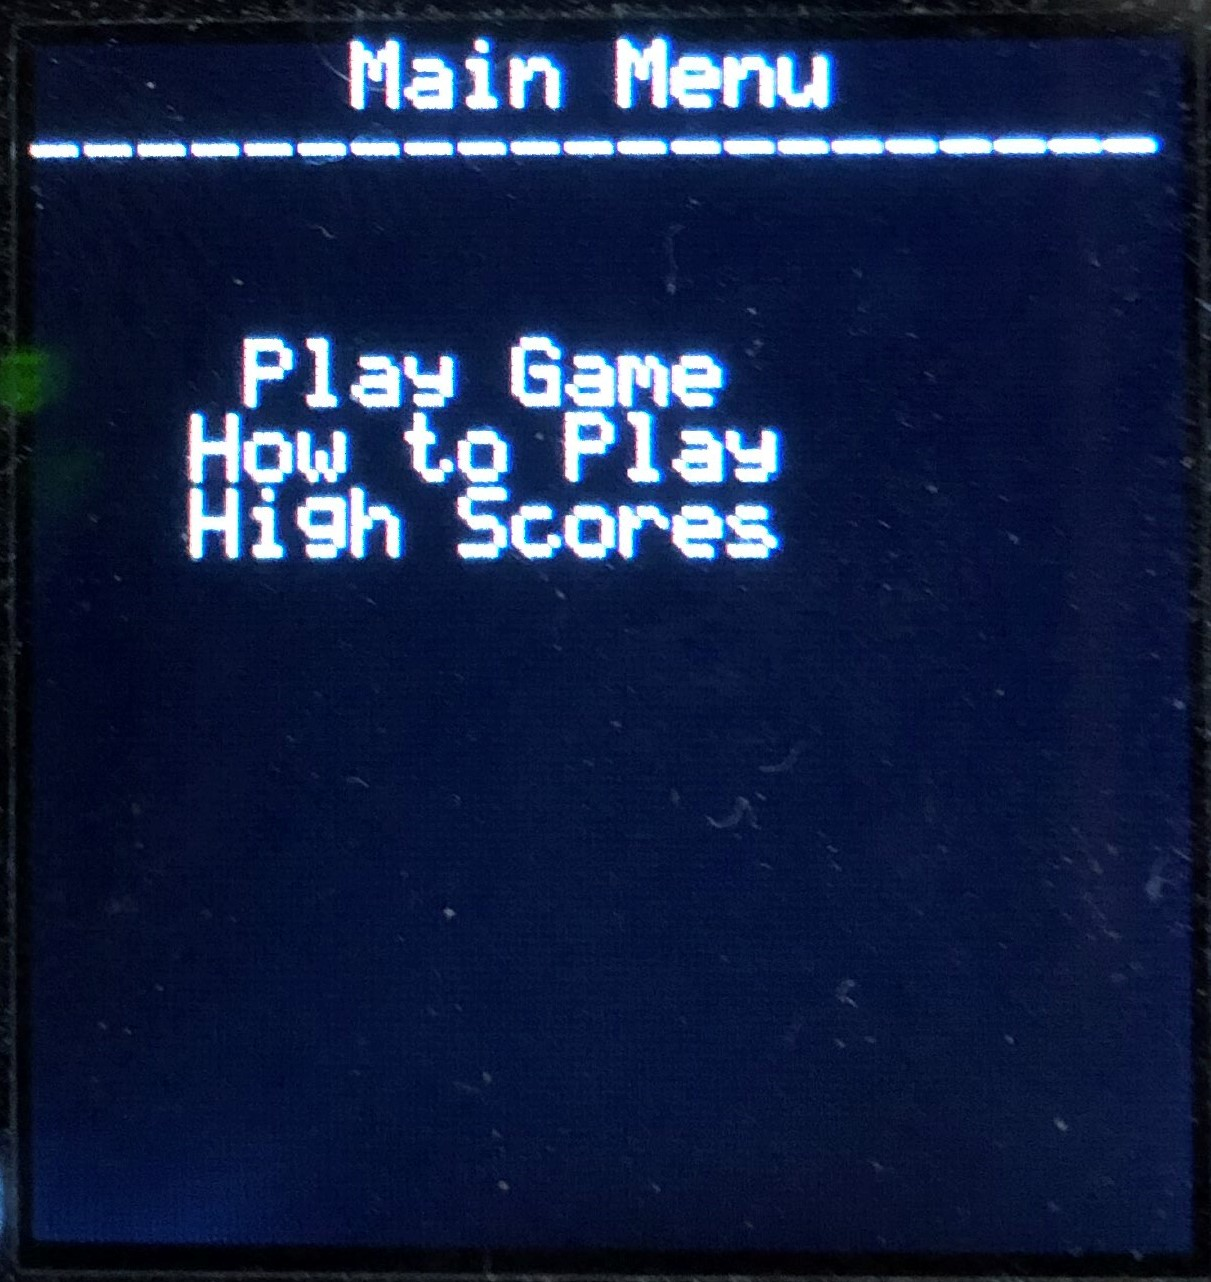
\includegraphics[width=.215\textwidth]{menu.jpg}}
    \boxed{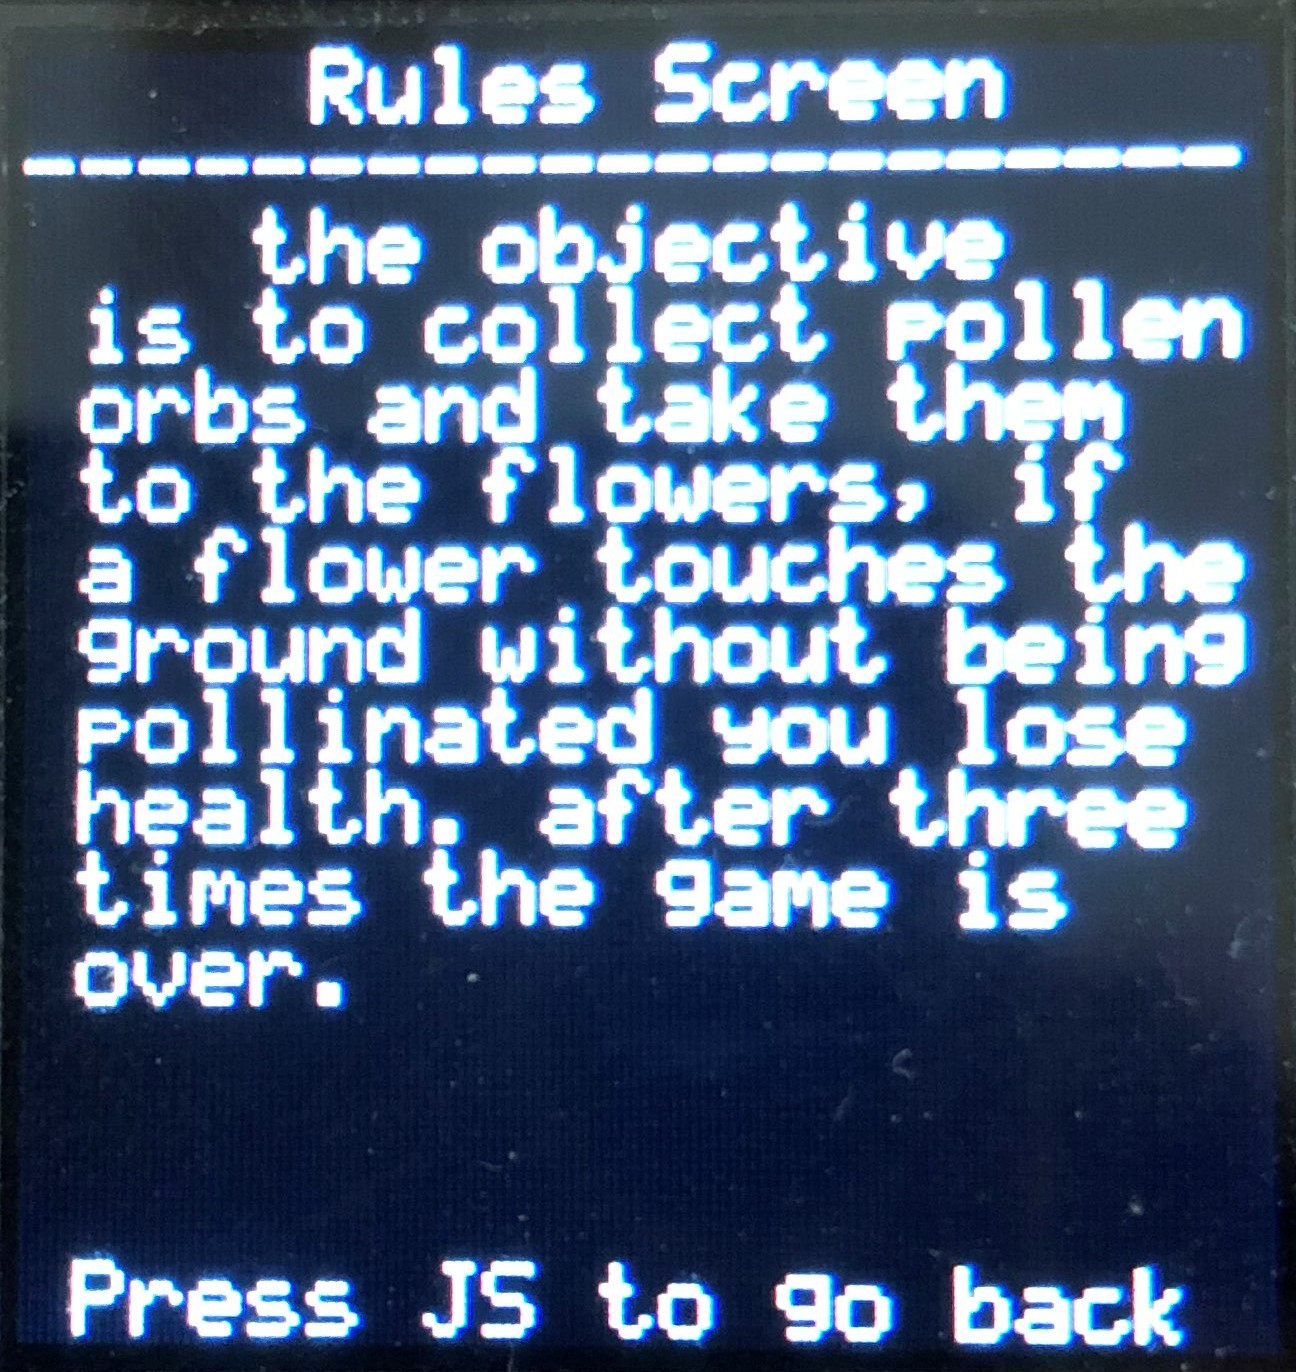
\includegraphics[width=.215\textwidth]{rules.jpg}}
    \boxed{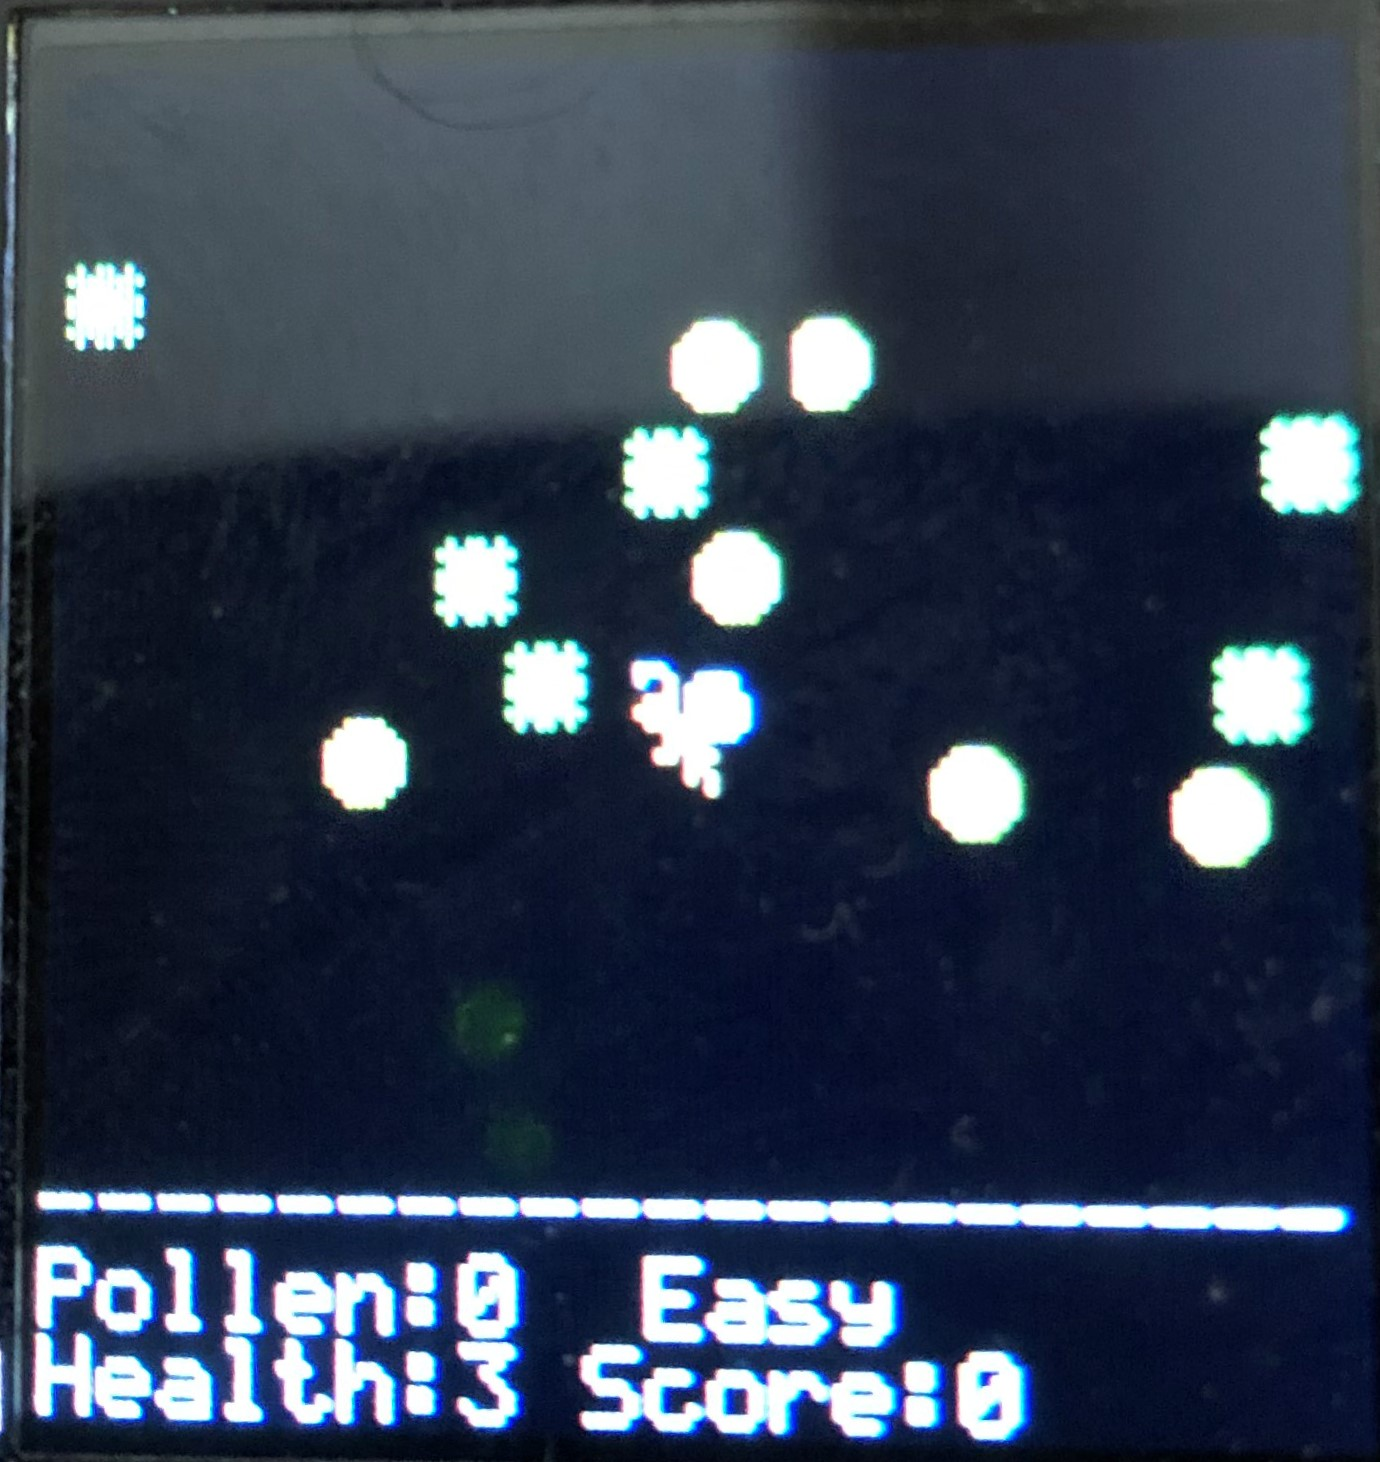
\includegraphics[width=.225\textwidth]{game.jpg}}
\end{center}

\section{Microcontroller-based embedded system architecture}
\begin{center}
    \begin{circuitikz}
    \draw (-2,0) node[draw,fill=pink,minimum width=40pt,minimum height=40pt](cpu){CPU}
    (-6,0) node[draw,fill=pink,minimum width=40pt,minimum height=40pt](msp){MSP}
    node[fit={(-3,-3)(3,3)},label={chip-level architecture},draw,inner sep=15pt]{}
    (-2,-2.5) node[draw,fill=pink,minimum size= 22.5pt](io1){I/O}
    (-1,-2.5) node[draw,fill=pink,minimum size= 22.5pt](io2){I/O}
    (0,-2.5) node[draw,fill=pink,minimum size= 22.5pt](io3){I/O}
    (1,-2.5) node[draw,fill=pink,minimum size= 22.5pt](io4){I/O}
    (2,-2.5) node[draw,fill=pink,minimum size= 22.5pt](io5){I/O}
    (0,2.5) node[draw,fill=pink,minimum size= 22.5pt](io6){I/O}
    (2,2.5) node[draw,fill=pink,minimum size= 22.5pt](io7){I/O}
    (0,1) node[draw,fill=pink,minimum width=30pt,minimum height=30pt](rx){$\begin{array}{c}euSCI\\RX\end{array}$}
    (2,1) node[draw,fill=pink,minimum width=30pt,minimum height=30pt](tx){$\begin{array}{c}euSCI\\TX\end{array}$}
    (cpu) to [short](io1)
    ($(cpu)+(.1,-.7)$) to [short]($(cpu)+(.1,-2)$)[short] to [short]($(cpu)+(1,-2)$)to[short]($(io2)+(0,.4)$)
    ($(cpu)+(.2,-.7)$) to [short]($(cpu)+(.2,-1.9)$)[short] to [short]($(cpu)+(2,-1.9)$)to[short]($(io3)+(0,.4)$)
    ($(cpu)+(.3,-.7)$) to [short]($(cpu)+(.3,-1.8)$)[short] to [short]($(cpu)+(3,-1.8)$)to[short]($(io4)+(0,.4)$)
    ($(cpu)+(.4,-.7)$) to [short]($(cpu)+(.4,-1.7)$)[short] to [short]($(cpu)+(4,-1.7)$)to[short]($(io5)+(0,.4)$)
    (io1) to [short,-*] ($(io1)+(0,-1.03)$) node[anchor=north]{P1.0}
    (io2) to [short,-*] ($(io2)+(0,-1.03)$) node[anchor=north]{P1.1}
    (io3) to [short,-*] ($(io3)+(0,-1.03)$) node[anchor=north]{P1.2}
    (io4) to [short,-*] ($(io4)+(0,-1.03)$) node[anchor=north]{P3.5}
    (io5) to [short,-*] ($(io5)+(0,-1.03)$) node[anchor=north]{P2.0}
    ($(rx)+(0,-.55)$) to [short]($(cpu)+(2,0)$) to [short](cpu)
    ($(tx)+(0,-.55)$) to [short]($(cpu)+(4,-.1)$) to [short]($(cpu)+(.71,-.1)$)
    (io6) to[short](rx)
    (io7) to[short](tx)
    ($(io6)+(0,.4)$) to [short]($(io6)+(0,.8)$) to [short,-*]($(io6)+(3.53,.8)$)node[anchor=west]{P1.3}
    ($(io7)+(0,.4)$) to [short]($(io7)+(0,.5)$) to [short,-*]($(io7)+(1.53,.5)$)node[anchor=west]{P1.2}
    node[fit={(-11,-3)(-5,3)},label={board-level architecture},draw,inner sep=15pt]{}
    (-6,2)node[draw,circle,fill=pink](ll1){JSY}
    (-7.25,2)node[draw,circle,fill=pink](ll2){JSX}
    (-8.5,2)node[draw,circle,fill=pink](jsb){JSB}
    (-9.75,2)node[draw,circle,fill=pink](bb1){BB1}
    (-6,-3.5)node[draw,fill=pink,minimum width=20pt,minimum height=20pt](usb){USB} to [short]
    (-6,-2.5)node[draw,fill=pink,minimum width=20pt,minimum height=20pt](xds){XDS} to [short]
    (-6,-1.5)node[draw,fill=pink,minimum width=20pt,minimum height=20pt](iso){Isolation}
    (msp) to [short] (ll1);
    \draw ($(iso)+(.2,.34)$) to [short]($(iso)+(.2,.78)$);
    \draw ($(iso)+(-.2,.34)$) to [short]($(iso)+(-.2,.78)$);
    \draw ($(msp)+(-.1,.7)$) to [short]($(msp)+(-.1,1.4)$) to [short]($(msp)+(-1.25,1.4)$) to [short]($(msp)+(-1.25,1.5)$);
    \draw ($(msp)+(-.2,.7)$) to [short]($(msp)+(-.2,1.3)$) to [short]($(msp)+(-2.5,1.3)$) to [short]($(msp)+(-2.5,1.5)$);
    \draw ($(msp)+(-.3,.7)$) to [short]($(msp)+(-.3,1.2)$) to [short]($(msp)+(-3.75,1.2)$) to [short]($(msp)+(-3.75,1.5)$);
    \draw (-10,0) node[draw,fill=pink,minimum width=35pt,minimum height=35pt](lcd){LCD} to[short](msp);
    \end{circuitikz}
\end{center}
\begin{center}
    Assuming the two boards we have are one, the architecture of this system is quite simple, since a very low amount of inputs from the actual boards are used, most inputs come from the joystick, there is also UART which gets used for a bonus point opportunity which is probably the most complicated part about the architecture.
\end{center}
\newpage
\section{Code Quality}
\subsection{Comments}
\begin{center}
    The comments in my code show what each function does, the input and output of each function, and whenever a chunk of code is called there is a brief explanation of when the code will be called and what happens when the code does get called. 
\end{center}
\subsection{No Global Variables}
\begin{center}
    The only global variables used are the ones used for images which according to specification are allowed
\end{center}
\subsection{No Numeric Values}
\begin{center}
    all values are defined using macros, which explain the meaning of the number
\end{center}
\subsection{No Long Functions}
\begin{center}
    All functions are below max length and line number commented at the top of relevant functions.
\end{center}
\subsection{Using HAL} 
\begin{center}
    The HAL were used properly when needed.
\end{center}
\subsection{Non-Blocking Code}
\begin{center}
    In all places of the code the blocking test did in fact turn on the LED and therefore the code is nonblocking.
\end{center}
\begin{center}
    \begin{tabular}{c|c}
         Code Quality Aspect &  Expected Points\\
         \hline
         Comments & 10\\
         No Global Variables & 20\\
         No Numeric Values & 20\\
         No Long Functions & 30\\
         Non-Blocking Code & 20\\
    \end{tabular}
\end{center}
\newpage
\section{Bonus Points}
\subsection{Difficulty Levels}
\begin{center}
    I added four difficulty levels, easy where its virutally impossible to lose, medium where it requires some forethought in where you go and which pollen you pickup, hard where it requires strategy to stay alive, and impossible, where its statistically impossible to win.
\end{center}
\subsection{Loading Bar on Title Screen}
\begin{center}
    I added a loading bar that moves from the bottom left of the screen to the right and is dynamic based on the input time. So if its 2 seconds, the bar will take two seconds and if its longer it will also be just as long
\end{center}
\subsection{Custom Titlescreen}
\begin{center}
    I added a bee animation of a bee flying on a sunny valley type thing hes kinda cute. The animation is also based on the amount of time, so the longer the wait time the longer the animation plays.
\end{center}
\subsection{Custom Graphics}
\begin{center}
    I added a custom bee player which turns left and right depending on which direction its moving in, custom unbloom flowers, custom bloom flowers and custom pollen (it doesnt show the pollen very well on the display but its not just a yellow circle theres shading on that it just dont work very well).
\end{center}
\subsection{Random Using ADC}
\begin{center}
    I factored the joystick movement into the seed for creating a random number, this way its much more random that it was originally since the psudorandom rand() function is based on time if something happens at the same point in time every time all object will spawn in the same place but since it was properly randomized there is nothing like that anymore.
\end{center}
\subsection{Analog Movement}
\begin{center}
    I had three "levels" of analog movement, the furthest from origin was fastest.
\end{center}
\begin{center}
    \begin{tabular}{c|c}
         Bonus Opportunities &  Expected Points\\
         \hline
         Difficulty Levels & 100\\
         Loading bar & 10\\
         Custom title & 30\\
         Custom graphics & 80\\
         Random Using ADC & 40\\
         Analog Movement & 50\\
    \end{tabular}
\end{center}
\end{document}
